  \documentclass[12pt,a4paper,twoside,openright]{report}

  % =============================================================================
  % PACKAGES ET CONFIGURATIONS ESSENTIELLES
  % =============================================================================
  \usepackage[utf8]{inputenc}
  \usepackage[T1]{fontenc}
  \usepackage[french]{babel}
  \frenchsetup{StandardLists=true} % Empeche babel d'interferer avec enumitem
  \usepackage{lmodern}
  \usepackage[top=2.5cm, bottom=2.5cm, left=3cm, right=2.5cm, headheight=20pt]{geometry}
  \usepackage{setspace}
  \onehalfspacing % Interligne standard de 1.5 pour memoire de PFE

  \usepackage{graphicx}
  \graphicspath{{figures/}{docs/figures/}{../docs/figures/}{./}}
  \usepackage{xcolor}
  \usepackage{amsmath,amssymb}
  \usepackage{booktabs}
  \usepackage{longtable}
  \usepackage{tabularx}
  \usepackage{array}
  \usepackage{fancyhdr}
  \usepackage{titlesec}
  \usepackage{enumitem}
  \usepackage[most]{tcolorbox}
  \usepackage{listings}
  \usepackage{microtype}
  \usepackage[font=small,labelfont=bf,labelsep=colon]{caption}
  \usepackage{float}
  \usepackage{url}

  % =============================================================================
  % PALETTE GRAPHIQUE PROFESSIONNELLE & ACADEMIQUE
  % =============================================================================
  \definecolor{primaryNavy}{RGB}{14, 34, 61}       % Bleu Nuit Institutionnel
  \definecolor{secondaryBlue}{RGB}{24, 76, 120}    % Bleu Academique
  \definecolor{accentCyan}{RGB}{13, 148, 136}      % Cyan Technique
  \definecolor{darkSlate}{RGB}{45, 55, 72}        % Gris Anthracite Titres
  \definecolor{lightBg}{RGB}{248, 250, 252}        % Fond doux encadres
  \definecolor{borderLight}{RGB}{226, 232, 240}    % Bordure encadres
  \definecolor{codeBg}{RGB}{241, 245, 249}         % Fond blocs de code
  \definecolor{successGreen}{RGB}{22, 101, 52}     % Succes / Validation
  \definecolor{warningOrange}{RGB}{194, 65, 12}    % Alertes
  \definecolor{crimsonDark}{RGB}{153, 27, 27}      % Points critiques

  % Symbole de puce personnalise robuste
  \newcommand{\itembullet}{\textcolor{secondaryBlue}{$\blacktriangleright$}}

  % Hyperref avec liens discrets et professionnels (sans pilote rigide)
  \usepackage[
      colorlinks=true,
      linkcolor=primaryNavy,
      citecolor=secondaryBlue,
      urlcolor=accentCyan,
      pdftitle={Rapport de Projet de Fin d'Etudes - AutoCare-AI},
      pdfauthor={FARIDI Marwane},
      pdfsubject={Diplome d'Ingenieur d'Etat en Genie Informatique - UPF}
  ]{hyperref}

  % =============================================================================
  % CONFIGURATION DES EN-TETES ET PIEDS DE PAGE (FANCYHDR)
  % =============================================================================
  \pagestyle{fancy}
  \fancyhf{}
  \fancyhead[LE,RO]{\small\color{darkSlate}\textit{\rightmark}}
  \fancyhead[LO,RE]{\small\color{darkSlate}\textit{\leftmark}}
  \fancyfoot[LE,RO]{\bfseries\color{primaryNavy}\thepage}
  \fancyfoot[LO,RE]{\small\color{gray}AutoCare-AI --- PFE UPF / NewDev}
  \renewcommand{\headrulewidth}{0.5pt}
  \renewcommand{\footrulewidth}{0.4pt}

  % Style pour les debuts de chapitre
  \fancypagestyle{plain}{
    \fancyhf{}
    \fancyfoot[C]{\bfseries\color{primaryNavy}\thepage}
    \renewcommand{\headrulewidth}{0pt}
    \renewcommand{\footrulewidth}{0pt}
  }

  % =============================================================================
  % DESIGN DES TITRES DE CHAPITRES ET SECTIONS (TITLESEC)
  % =============================================================================
  \titleformat{\chapter}[display]
    {\normalfont\bfseries\color{primaryNavy}}
    {\filleft\small\bfseries\color{accentCyan}\MakeUppercase{Chapitre}\ \Huge\color{secondaryBlue}\thechapter}
    {1.5ex}
    {\Huge}
    [\vspace{1.5ex}{\color{secondaryBlue}\titlerule[1.2pt]}]

  \titleformat{name=\chapter,numberless}[block]
    {\normalfont\bfseries\color{primaryNavy}\Huge}
    {}
    {0pt}
    {}
    [\vspace{1.5ex}{\color{secondaryBlue}\titlerule[1.2pt]}]

  \titlespacing*{\chapter}{0pt}{-10pt}{25pt}
  \titlespacing*{name=\chapter,numberless}{0pt}{-10pt}{20pt}
  \titlespacing*{\section}{0pt}{16pt}{8pt}
  \titlespacing*{\subsection}{0pt}{12pt}{6pt}
  \titlespacing*{\subsubsection}{0pt}{10pt}{4pt}

  \titleformat{\section}
    {\normalfont\Large\bfseries\color{primaryNavy}}
    {\color{secondaryBlue}\thesection}{1em}{}

  \titleformat{\subsection}
    {\normalfont\large\bfseries\color{secondaryBlue}}
    {\color{accentCyan}\thesubsection}{1em}{}

  \titleformat{\subsubsection}
    {\normalfont\normalsize\bfseries\color{darkSlate}}
    {\thesubsubsection}{1em}{}

  % =============================================================================
  % BOITES D'ENCADRES MODERNES (TCOLORBOX)
  % =============================================================================
  \newtcolorbox{infoBox}[1][]{
    colback=lightBg,
    colframe=secondaryBlue,
    fonttitle=\bfseries\color{white},
    coltitle=white,
    title={#1},
    arc=2.5mm,
    boxrule=0.8pt,
    left=12pt, right=12pt, top=10pt, bottom=10pt
  }

  \newtcolorbox{problemBox}[1][]{
    colback=white,
    colframe=crimsonDark,
    fonttitle=\bfseries\color{white},
    coltitle=white,
    title={\textbf{Probl\'ematique M\'etier : #1}},
    arc=2mm,
    boxrule=1pt,
    left=12pt, right=12pt, top=9pt, bottom=9pt
  }

  \newtcolorbox{techDecision}[1][]{
    colback=lightBg,
    colframe=primaryNavy,
    fonttitle=\bfseries\color{white},
    coltitle=white,
    title={\textbf{D\'ecision d'Architecture : #1}},
    arc=2mm,
    boxrule=1pt,
    left=12pt, right=12pt, top=9pt, bottom=9pt
  }

  \newtcolorbox{sprintBox}[1][]{
    colback=white,
    colframe=accentCyan,
    fonttitle=\bfseries\color{white},
    coltitle=white,
    title={\textbf{Synth\`ese de Sprint Agile : #1}},
    arc=2mm,
    boxrule=0.8pt,
    left=10pt, right=10pt, top=8pt, bottom=8pt
  }

  % =============================================================================
  % LISTINGS (CODE SOURCE)
  % =============================================================================
  \lstset{
    backgroundcolor=\color{codeBg},
    basicstyle=\footnotesize\ttfamily\color{darkSlate},
    breakatwhitespace=false,
    breaklines=true,
    captionpos=b,
    commentstyle=\color{successGreen}\itshape,
    keywordstyle=\color{primaryNavy}\bfseries,
    stringstyle=\color{warningOrange},
    numbers=left,
    numberstyle=\tiny\color{gray},
    stepnumber=1,
    numbersep=8pt,
    showspaces=false,
    showstringspaces=false,
    showtabs=false,
    frame=single,
    rulecolor=\color{borderLight},
    tabsize=2,
    inputencoding=utf8,
    extendedchars=true
  }

  % =============================================================================
  % MACRO D'INSERTION D'IMAGES / DIAGRAMMES RESILIENTE
  % =============================================================================
  \newcommand{\insertdiagramme}[4][width=0.88\textwidth]{%
    \begin{figure}[htbp]%
      \centering%
      \IfFileExists{#2}{%
        \includegraphics[#1]{#2}%
      }{%
        \IfFileExists{figures/#2}{%
          \includegraphics[#1]{figures/#2}%
        }{%
          \IfFileExists{docs/#2}{%
            \includegraphics[#1]{docs/#2}%
          }{%
            \fcolorbox{secondaryBlue}{lightBg}{%
              \begin{minipage}{0.88\textwidth}%
                \centering\vspace{1cm}%
                {\color{secondaryBlue}\Large\bfseries [ Emplacement Figure / Diagramme ]}\\[0.35cm]%
                {\small\bfseries\color{primaryNavy} #3}\\[0.25cm]%
                {\footnotesize\color{darkSlate}\textit{Image attendue dans \texttt{docs/figures/}}}\\[0.15cm]%
                {\scriptsize\color{gray}\textit{(D\'eposez votre diagramme export\'e au format PNG/JPG sous ce nom)}}\vspace{1cm}%
              \end{minipage}%
            }%
          }%
        }%
      }%
      \caption{#3}%
      \label{#4}%
    \end{figure}%
  }

  % =============================================================================
  % DEBUT DU DOCUMENT
  % =============================================================================
  \begin{document}

  % =============================================================================
  % PAGE DE GARDE OFFICIELLE PFE
  % =============================================================================
  \begin{titlepage}
    \vspace*{-1cm}
    \noindent
    \begin{minipage}[t]{0.48\textwidth}
      \begin{flushleft}
        \textbf{\large UNIVERSIT\'E PRIV\'EE DE F\`ES}\\[0.1cm]
        \small Facult\'e des Sciences de l'Ing\'enieur\\[0.1cm]
        \footnotesize Fili\`ere : G\'enie Informatique\\[0.3cm]
        \IfFileExists{figures/logo_upf.png}{
\includegraphics[height=1.8cm]{figures/logo_upf.png}}{\IfFileExists{docs/figures/logo_upf.png}{
\includegraphics[height=1.8cm]{docs/figures/logo_upf.png}}{\fbox{\textbf{Logo UPF}}}}
      \end{flushleft}
    \end{minipage}
    \hfill
    \begin{minipage}[t]{0.48\textwidth}
      \begin{flushright}
        \textbf{\large NEWDEV STARTUP}\\[0.1cm]
        \small P\^ole Ing\'enierie Logicielle \& IA\\[0.1cm]
        \footnotesize Casablanca, Maroc\\[0.3cm]
        \IfFileExists{figures/logo_newdev.png}{\includegraphics[height=1.8cm]{figures/logo_newdev.png}}{\IfFileExists{docs/figures/logo_newdev.png}{\includegraphics[height=1.8cm]{docs/figures/logo_newdev.png}}{\fbox{\textbf{Logo NewDev}}}}
      \end{flushright}
    \end{minipage}

    \vspace{1.5cm}
    \begin{center}
      {\large\scshape\bfseries M\'emoire de Projet de Fin d'\'Etudes}\\[0.3cm]
      {\normalsize En vue de l'obtention du}\\[0.2cm]
      {\large\bfseries\color{secondaryBlue} Dipl\^ome d'Ing\'enieur d'\'Etat en G\'enie Informatique}\\[1.2cm]

      \begin{tcolorbox}[colback=primaryNavy!5,colframe=primaryNavy,arc=3mm,boxrule=1.5pt,width=\textwidth,halign=center]
        \vspace{0.3cm}
        {\Huge\bfseries\color{primaryNavy} AutoCare-AI}\\[0.35cm]
        {\large\bfseries\color{secondaryBlue} Conception et R\'ealisation d'une Plateforme Intelligente de Maintenance Pr\'edictive et de Jumelage Num\'erique Automobile}
        \vspace{0.3cm}
      \end{tcolorbox}

      \vspace{1.8cm}

      \noindent
      \begin{minipage}[t]{0.48\textwidth}
        \begin{flushleft} \large
          \textbf{\color{primaryNavy}R\'ealis\'e par :}\\[0.15cm]
          \textbf{M. FARIDI Marwane}\\[0.1cm]
          \small \'El\`eve Ing\'enieur en G\'enie Informatique
        \end{flushleft}
      \end{minipage}
      \hfill
      \begin{minipage}[t]{0.48\textwidth}
        \begin{flushright} \large
          \textbf{\color{primaryNavy}Encadr\'e par :}\\[0.15cm]
          \textbf{M. Mohamed HAJJOUJI}\\[0.1cm]
          \small Encadrant Professionnel --- NewDev
        \end{flushright}
      \end{minipage}

      \vfill
      {\color{secondaryBlue}\rule{0.65\textwidth}{0.8pt}}\\[0.25cm]
      {\bfseries\color{darkSlate} Ann\'ee Universitaire : 2025 -- 2026}
    \end{center}
  \end{titlepage}

  % =============================================================================
  % NUMEROTATION ROMAINE POUR PAGES PRELIMINAIRES
  % =============================================================================
  \pagenumbering{roman}
  \setcounter{page}{1}

  % =============================================================================
  % DEDICACES
  % =============================================================================
  \chapter*{D\'edicaces}
  \addcontentsline{toc}{chapter}{D\'edicaces}

  \vspace{1cm}
  \begin{flushright}
    \itshape
    \`A mes chers parents,\\
    pour leurs sacrifices inestimables, leur amour inconditionnel\\
    et leurs pri\`eres qui m'ont \'eclair\'e le chemin tout au long de mes \'etudes.\\[0.8cm]
    
    \`A ma famille et mes proches,\\
    pour leur soutien ind\'efectible, leur confiance et leurs encouragements constants.\\[0.8cm]
    
    \`A mes professeurs et ma\^itres de l'Universit\'e Priv\'ee de F\`es,\\
    qui ont forg\'e mes comp\'etences avec rigueur et d\'evouement.\\[0.8cm]
    
    \`A tous ceux qui ont contribu\'e, de pr\`es ou de loin,\\
    \`a l'accomplissement de ce travail.\\
    
    \vspace{1cm}
    \textbf{FARIDI Marwane}
  \end{flushright}

  \newpage

  % =============================================================================
  % REMERCIEMENTS
  % =============================================================================
  \chapter*{Remerciements}
  \addcontentsline{toc}{chapter}{Remerciements}

  Ce travail de fin d'\'etudes n'aurait pu voir le jour sans le soutien, l'orientation et la bienveillance de nombreuses personnes auxquelles je tiens \`a exprimer ma profonde gratitude.

  Je tiens tout d'abord \`a remercier chaleureusement mon encadrant professionnel chez \textbf{NewDev}, \textbf{Monsieur Mohamed HAJJOUJI}, pour son accueil, sa disponibilit\'e exemplaire, ses conseils avis\'es et la confiance qu'il m'a accord\'ee tout au long de ce stage. Ses orientations techniques exigeantes et sa vision industrielle ont \'et\'e des moteurs essentiels dans la maturation du projet \textbf{AutoCare-AI}.

  J'adresse \'egalement mes vifs remerciements \`a l'ensemble de l'\'equipe de \textbf{NewDev} pour l'environnement stimulant, collaboratif et bienveillant dans lequel j'ai eu l'opportunit\'e d'\'evoluer, ainsi que pour les pr\'ecieux partages d'exp\'erience en mati\`ere d'ing\'enierie logicielle et de solutions cloud.

  Mes remerciements s'adressent avec respect au corps professoral et \`a la direction p\'edagogique du d\'epartement \textbf{G\'enie Informatique} de l'\textbf{Universit\'e Priv\'ee de F\`es (UPF)}, pour la qualit\'e de l'enseignement dispens\'e et le socle acad\'emique solide dont j'ai b\'en\'efici\'e au long de mon cursus d'ing\'enieur.

  Enfin, je remercie tr\`es sinc\`erement les honorables membres du jury qui me font l'honneur d'\'evaluer ce travail et d'enrichir ce m\'emoire par leurs observations et critiques constructives.

  \newpage

  % =============================================================================
  % RESUME & ABSTRACT
  % =============================================================================
  \chapter*{R\'esum\'e}
  \addcontentsline{toc}{chapter}{R\'esum\'e}

  La gestion et la maintenance des v\'ehicules automobiles demeurent largement tributaires de processus curatifs et r\'eactifs, entra\^inant des pannes impr\'evues, des co\^uts de r\'eparation disproportionn\'es et un manque d'anticipation budg\'etaire pour les propri\'etaires et gestionnaires de flottes. Ce Projet de Fin d'\'Etudes, r\'ealis\'e au sein de la startup \textbf{NewDev}, a pour objectif la conception et l'impl\'ementation d'une plateforme SaaS compl\`ete de maintenance pr\'edictive et de jumelage num\'erique automobile, baptis\'ee \textbf{AutoCare-AI}.

  La solution repose sur une architecture d\'ecoupl\'ee robuste articul\'ee autour d'un backend \textbf{Spring Boot 3} sous \textbf{Java 21}, d'une base relationnelle \textbf{PostgreSQL}, d'une application mobile cross-platform haute performance d\'evelopp\'ee avec \textbf{React Native / Expo}, et d'une interface d'administration sous \textbf{React}. Le c\oe ur technologique int\`egre un moteur de jumelage num\'erique (\textit{Digital Twin}) \'evaluant l'usure dynamique des organes critiques (freinage, suspension, lubrification, transmission) en croisant t\'el\'em\'etrie, mill\'esime et conditions d'usage. Ce moteur est coupl\'e \`a des mod\`eles g\'en\'eratifs et analytiques \textbf{Google Gemini AI} permettant de fournir des diagnostics probabilistes en langage naturel, des pr\'econisations d'entretien prioris\'ees et des projections budg\'etaires intelligentes \`a 3, 6 et 12 mois. La s\'ecurit\'e est assur\'ee par un protocole sans \'etat bas\'e sur des jetons JWT et une politique stricte de rotation et r\'evocation des Refresh Tokens multi-terminaux.

  \vspace{0.5cm}
  \noindent\textbf{Mots-cl\'es :} Maintenance Pr\'edictive, Jumelage Num\'erique (Digital Twin), Intelligence Artificielle, Spring Boot 3, React Native, Google Gemini, S\'ecurit\'e JWT, PostgreSQL.

  \vspace{1.5cm}

  \chapter*{Abstract}
  \addcontentsline{toc}{chapter}{Abstract}

  Automotive maintenance operations have traditionally relied on reactive and curative paradigms, resulting in unexpected mechanical failures, prohibitive repair expenses, and poor budget planning for vehicle owners and fleet managers. This Master's thesis / Engineering capstone project, conducted at the startup \textbf{NewDev}, delivers the end-to-end design and realization of a comprehensive automotive predictive maintenance and digital twin platform named \textbf{AutoCare-AI}.

  The solution features a decoupled, multi-tier architecture powered by a \textbf{Spring Boot 3} backend on \textbf{Java 21}, a \textbf{PostgreSQL} enterprise database, an ergonomic cross-platform mobile application developed with \textbf{React Native / Expo}, and a \textbf{React} administration dashboard. The technical core integrates a \textit{Digital Twin} engine assessing component degradation across critical automotive systems (braking, suspension, powertrain, lubrication) by correlating telemetry, mileage, and driving environments. This algorithm interfaces with \textbf{Google Gemini AI} to deliver contextualized natural-language diagnostics, prioritized maintenance advisories, and predictive budget forecasting for 3, 6, and 12-month periods. End-to-end security is guaranteed through a stateless JWT authentication framework complemented by multi-device refresh token rotation and revocation.

  \vspace{0.5cm}
  \noindent\textbf{Keywords:} Predictive Maintenance, Digital Twin, Artificial Intelligence, Spring Boot 3, React Native, Google Gemini, JWT Security, PostgreSQL.

  \newpage

  % =============================================================================
  % TABLES DES MATIERES, FIGURES ET TABLEAUX
  % =============================================================================
  \tableofcontents
  \newpage
  \listoffigures
  \newpage
  \listoftables
  \newpage

  % =============================================================================
  % LISTE DES ABREVIATIONS ET ACRONYMES
  % =============================================================================
  \chapter*{Liste des Sigles et Acronymes}
  \addcontentsline{toc}{chapter}{Liste des Sigles et Acronymes}

  \begin{longtable}{p{0.25\textwidth} p{0.70\textwidth}}
  \toprule
  \textbf{Acronyme} & \textbf{D\'efinition Compl\`ete} \\
  \midrule
  \endhead
  \textbf{API} & Application Programming Interface \\
  \textbf{ASCII} & American Standard Code for Information Interchange \\
  \textbf{BCrypt} & Blowfish-based Password Cryptographic Hashing Function \\
  \textbf{BDD} & Base de Donn\'ees Relationnelle \\
  \textbf{BLE} & Bluetooth Low Energy \\
  \textbf{CI/CD} & Continuous Integration / Continuous Deployment \\
  \textbf{CORS} & Cross-Origin Resource Sharing \\
  \textbf{CRUD} & Create, Read, Update, Delete \\
  \textbf{CSRF} & Cross-Site Request Forgery \\
  \textbf{DTO} & Data Transfer Object \\
  \textbf{E.164} & Format international standard de num\'erotation t\'el\'ephonique \\
  \textbf{GPS} & Global Positioning System \\
  \textbf{HTML} & HyperText Markup Language \\
  \textbf{HTTP / HTTPS} & HyperText Transfer Protocol / HTTP Secure \\
  \textbf{IDE} & Integrated Development Environment \\
  \textbf{I18n} & Internationalisation (support multilingue) \\
  \textbf{JPA} & Java Persistence API \\
  \textbf{JSON} & JavaScript Object Notation \\
  \textbf{JWT} & JSON Web Token \\
  \textbf{LLM} & Large Language Model \\
  \textbf{MVC} & Mod\`ele-Vue-Contr\^oleur \\
  \textbf{OBD-II} & On-Board Diagnostics version 2 (Prise diagnostique v\'ehicule) \\
  \textbf{OEM} & Original Equipment Manufacturer (Constructeur Automobile) \\
  \textbf{ORM} & Object-Relational Mapping \\
  \textbf{PFE} & Projet de Fin d'\'Etudes \\
  \textbf{REST} & Representational State Transfer \\
  \textbf{RGPD} & R\`eglement G\'en\'eral sur la Protection des Donn\'ees \\
  \textbf{RTL} & Right-To-Left (Lecture de droite \`a gauche, e.g., Arabe) \\
  \textbf{SaaS} & Software as a Service \\
  \textbf{SDK} & Software Development Kit \\
  \textbf{SPA} & Single Page Application \\
  \textbf{SQL} & Structured Query Language \\
  \textbf{UML} & Unified Modeling Language \\
  \textbf{UPF} & Universit\'e Priv\'ee de F\`es \\
  \textbf{UUID} & Universally Unique Identifier \\
  \textbf{VIN} & Vehicle Identification Number (Num\'ero de s\'erie ch\^assis) \\
  \textbf{XSS} & Cross-Site Scripting \\
  \bottomrule
  \end{longtable}

  \newpage

  % =============================================================================
  % CORPS DU MEMOIRE (NUMEROTATION ARABE)
  % =============================================================================
  \pagenumbering{arabic}
  \setcounter{page}{1}

  % =============================================================================
  % INTRODUCTION GENERALE
  % =============================================================================
  \chapter*{Introduction G\'en\'erale}
  \addcontentsline{toc}{chapter}{Introduction G\'en\'erale}

  L'industrie automobile traverse aujourd'hui l'une des mutations technologiques les plus profondes de son histoire. Port\'ee par la prolif\'eration des capteurs embarqu\'es, la connectivit\'e permanente et l'essor de l'Intelligence Artificielle, l'automobile moderne ne se d\'efinit plus uniquement comme un bien m\'ecanique mat\'eriel, mais comme un syst\`eme cyber-physique communicant et g\'en\'erateur de volumes massifs de donn\'ees t\'el\'em\'etriques.

  Pourtant, en d\'epit de cette sophistication technologique croissante, la gestion de l'entretien et du suivi m\'ecanique pour la majorit\'e des automobilistes et des petites flottes d'entreprise demeure ancr\'ee dans des approches anachroniques. Les d\'emarches curatives dominent : l'automobiliste attend g\'en\'eralement la manifestation d'une panne critique, l'apparition d'un voyant d'anomalie sur le combin\'e de bord ou le refus du contr\^ole technique p\'eriodique pour r\'eagir. Cette gestion r\'eactive engendre des cons\'equences n\'egatives manifestes :
  \begin{itemize}[label=\itembullet]
    \item \textbf{Surco\^uts financiers majeurs :} une anomalie mineure non d\'etect\'ee (telle qu'une usure asym\'etrique des plaquettes ou une d\'egradation pr\'ecoce de l'indice de viscosit\'e d'huile) se propage rapidement aux organes adjacents, provoquant des r\'eparations lourdes (disques voil\'es, casse turbo, avarie moteur).
    \item \textbf{Risques accrus pour la s\'ecurit\'e routi\`ere :} la d\'efaillance inopin\'ee d'un composant de liaison au sol ou du syst\`eme de freinage compromet directement la s\'ecurit\'e des passagers.
    \item \textbf{Impr\'evisibilit\'e budg\'etaire :} l'incapacit\'e d'anticiper les \'ech\'eances d'entretien et le renouvellement des pi\`eces d'usure d\'estabilise le budget des m\'enages et la tr\'esorerie des gestionnaires.
  \end{itemize}

  Face \`a ces enjeux, la transition vers la \textbf{maintenance pr\'edictive} et le concept de \textbf{Jumelage Num\'erique (\textit{Digital Twin})} s'impose comme une r\'eponse d'ing\'enierie particuli\`erement pertinente. En cr\'eant un r\'eplica virtuel en temps r\'eel du v\'ehicule, aliment\'e par ses caract\'eristiques intrins\`eques, son historique d'intervention, son kilom\'etrage et l'analyse continue par intelligence artificielle, il devient possible d'anticiper les d\'egradations mat\'erielles avant qu'elles n'entra\^inent des dommages critiques.

  C'est dans ce cadre d'innovation appliqu\'ee que s'inscrit ce Projet de Fin d'\'Etudes, r\'ealis\'e au sein de la startup technologique \textbf{NewDev}. L'objectif central est de concevoir et de r\'ealiser la plateforme logicielle \textbf{AutoCare-AI}, un \'ecosyst\`eme complet compos\'e :
  \begin{enumerate}
    \item D'un moteur backend d'ing\'enierie et d'API REST sous \textbf{Spring Boot 3 / Java 21}, garantissant scalabilit\'e, haute s\'ecurit\'e des acc\`es et persistance relationnelle sous \textbf{PostgreSQL}.
    \item D'une application mobile moderne sous \textbf{React Native / Expo}, offrant aux automobilistes une ergonomie inspir\'ee des interfaces OEM premium (mode sombre \'el\'egant, affichage t\'el\'em\'etrique, gestion multilingue avec support RTL).
    \item D'un moteur d'intelligence artificielle aliment\'e par \textbf{Google Gemini AI}, charg\'e d'analyser l'usure, de g\'en\'erer des recommandations proactives et de calculer des pr\'evisions budg\'etaires personnalis\'ees \`a 3, 6 et 12 mois.
    \item D'un portail web d'administration pour la gouvernance de la plateforme, la gestion des flottes et l'audit de s\'ecurit\'e.
  \end{enumerate}

  Le pr\'esent m\'emoire s'organise en six chapitres structur\'es selon les normes acad\'emiques et professionnelles de l'ing\'enierie logicielle :
  \begin{itemize}[label=\itembullet]
    \item Le \textbf{Chapitre 1} pose le contexte g\'en\'eral du projet, pr\'esente la structure d'accueil \textbf{NewDev}, analyse la probl\'ematique m\'etier et expose la d\'emarche m\'ethodologique Agile/Scrum adopt\'ee.
    \item Le \textbf{Chapitre 2} d\'etaille l'analyse et la sp\'ecification des besoins, formalisant les exigences fonctionnelles et non-fonctionnelles de l'\'ecosyst\`eme.
    \item Le \textbf{Chapitre 3} pr\'esente la conception et la mod\'elisation UML du syst\`eme (cas d'utilisation, diagrammes de s\'equence critiques, diagramme de classes) ainsi que la mod\'elisation de la base de donn\'ees relationnelle.
    \item Le \textbf{Chapitre 4} \'etudie l'architecture logicielle globale et justifie de mani\`ere critique le choix des technologies backend, mobile, web et IA.
    \item Le \textbf{Chapitre 5} documente la r\'ealisation technique, l'impl\'ementation des algorithmes centraux et pr\'esente les interfaces utilisateurs r\'esultantes.
    \item Le \textbf{Chapitre 6} d\'etaille la strat\'egie d'assurance qualit\'e, les tests unitaires et d'int\'egration Spring Boot, ainsi que les perspectives de d\'eploiement continu.
  \end{itemize}

  Enfin, une conclusion g\'en\'erale dresse le bilan des r\'ealisations, \'evalue les comp\'etences d'ing\'enierie d\'evelopp\'ees et esquisse les \'evolutions futures de la plateforme.

  \newpage

  % =============================================================================
  % CHAPITRE 1 : CONTEXTE GENERAL & CONDUITE DE PROJET
  % =============================================================================
  \chapter{Contexte G\'en\'eral du Projet \& Conduite de Projet}

  \section{Introduction}
  Ce premier chapitre a pour vocation de situer le cadre g\'en\'eral dans lequel s'est d\'eroul\'e ce stage de fin d'\'etudes. Nous y pr\'esentons l'organisme d'accueil \textbf{NewDev}, analysons la probl\'ematique industrielle adress\'ee par le projet, dressons un \'etat de l'art concurrentiel et d\'etaillons la m\'ethodologie de gestion de projet adopt\'ee.

  \section{Pr\'esentation de l'Organisme d'Accueil : NewDev}
  \subsection{Identit\'e et Vocation}
  \textbf{NewDev} est une startup innovante sp\'ecialis\'ee dans le d\'eveloppement de solutions logicielles avanc\'ees, l'ing\'enierie cloud et l'int\'egration de technologies d'Intelligence Artificielle au service de la transformation num\'erique des entreprises. Fond\'ee par des ing\'enieurs passionn\'es, l'entreprise se distingue par une culture d'excellence technique, privil\'egiant des architectures logicielles propres (\textit{Clean Architecture}), modulaires et p\'erennes.

  \subsection{Domaines d'Expertise}
  Les activit\'es principales de NewDev s'articulent autour de plusieurs axes compl\'ementaires :
  \begin{itemize}[label=\itembullet]
    \item \textbf{Ing\'enierie Logicielle Sur-Mesure :} conception d'architectures d'entreprise r\'esilientes (microservices, API RESTful s\'ecuris\'ees, syst\`emes distribu\'es).
    \item \textbf{Applications Mobiles Cross-Platform :} d\'eveloppement d'exp\'eriences utilisateur performantes sous React Native et Flutter avec un haut niveau de fid\'elit\'e visuelle.
    \item \textbf{Intelligence Artificielle Appliqu\'ee :} int\'egration de mod\`eles de langage (LLM), de vision par ordinateur et d'algorithmes pr\'edictifs dans les processus m\'etiers.
    \item \textbf{DevOps \& Cloud Native :} automatisation de pipelines d'int\'egration et de d\'eploiement continus (CI/CD), conteneurisation et monitoring d'infrastructures.
  \end{itemize}

  \subsection{Cadre du Stage}
  Au sein du p\^ole R\&D de NewDev, notre mission consistait \`a piloter le cycle complet de conception et de r\'ealisation de la plateforme \textbf{AutoCare-AI}, sous la supervision directe de \textbf{M. Mohamed HAJJOUJI}. Cette immersion en startup a exig\'e polyvalence, rigueur dans le respect des standards industriels et capacit\'e \`a allier profondeur architecturale backend et r\'eactivit\'e ergonomique frontend.

  \section{Probl\'ematique M\'etier \& Motivation du Projet}
  \begin{problemBox}[La Maintenance Automobile R\'eactive et ses Limites]
  Le co\^ut moyen de possession d'un v\'ehicule automobile a progress\'e de plus de 25\,\% au cours de la derni\`ere d\'ecennie, port\'e par la complexit\'e technologique des sous-syst\`emes embarqu\'es. Malgr\'e cela, 78\,\% des interventions m\'ecaniques sont d\'eclench\'ees apr\`es l'apparition d'une d\'efaillance av\'er\'ee. Cette approche engendre une cascade de dysfonctionnements, un sentiment de m\'efiance envers les ateliers de r\'eparation et une gestion budg\'etaire anarchique pour les usagers.
  \end{problemBox}

  L'analyse du secteur automobile r\'ev\`ele plusieurs d\'efaillances structurelles :
  \begin{enumerate}
    \item \textbf{L'asym\'etrie d'information :} le propri\'etaire moyen est incapable d'estimer avec pr\'ecision le degr\'e d'usure de ses disques de freins, de ses suspensions ou de son fluide de bo\^ite de vitesses entre deux entretiens espac\'es.
    \item \textbf{L'obsolescence des carnets d'entretien physiques :} les carnets papier sont fr\'equemment \'egar\'es, mal renseign\'es ou falsifi\'es lors des reventes de v\'ehicules d'occasion.
    \item \textbf{L'absence de personnalisation des p\'eriodicit\'es :} les pr\'econisations constructeurs sont statiques (e.g., vidange tous les 15\,000 km) et ignorent les conditions r\'eelles d'usage (trajets urbains courts avec cycles thermiques s\'ev\`eres versus autoroute fluide, climat aride, poussi\`ere).
    \item \textbf{L'impr\'evisibilit\'e des flux financiers :} les pannes majeures surviennent sans pr\'eavis, imposant des d\'epenses impr\'evues souvent \'elev\'ees.
  \end{enumerate}

  Le projet \textbf{AutoCare-AI} r\'epond pr\'ecis\'ement \`a cette \'equation en fournissant un outil intelligent permettant de transformer chaque v\'ehicule en un \textbf{Jumeau Num\'erique} pr\'edictif, capable de simuler son usure, de recommander les op\'erations n\'ecessaires au moment optimal et d'estimer les budgets futurs avec pr\'ecision.

  \section{\'Etude de l'Existant \& Analyse Concurrentielle}
  Pour positionner \textbf{AutoCare-AI} de mani\`ere innovante sur le march\'e, une \'etude comparative des solutions existantes a \'et\'e men\'ee. Le tableau~\ref{tab:benchmark} synth\'etise cette analyse.

  \begin{table}[H]
  \centering
  \small
  \begin{tabularx}{\textwidth}{p{3.2cm} X X X}
  \toprule
  \textbf{Crit\`ere d'\'Evaluation} & \textbf{Solutions OBD Traditionnelles (e.g. Carly, Torque)} & \textbf{Applications de D\'epenses (e.g. Drivvo, Fuelio)} & \textbf{AutoCare-AI (Notre Solution)} \\
  \midrule
  \textbf{Approche Maintenance} & R\'eactive (lecture de codes d\'efauts DTC une fois apparus). & Passive (simple journalisation manuelle des co\^uts pass\'es). & \textbf{Pr\'edictive \& Proactive (anticipation avant d\'efaillance).} \\
  \addlinespace
  \textbf{Jumelage Num\'erique} & Inexistant (simple affichage de jauges instantan\'ees). & Aucun. & \textbf{Moteur Digital Twin complet mod\'elisant chaque sous-syst\`eme.} \\
  \addlinespace
  \textbf{Intelligence Artificielle} & Aucune (lexique statique de codes d'erreur). & Aucune. & \textbf{IA G\'en\'erative Gemini contextualis\'ee + Algorithmes d'usure.} \\
  \addlinespace
  \textbf{Planification Budg\'etaire} & Absente. & Statistiques basiques d'historique pass\'e. & \textbf{Projections pr\'edictives intelligentes \`a 3, 6 et 12 mois.} \\
  \addlinespace
  \textbf{Architecture S\'ecuris\'ee} & Mono-utilisateur, stockage local majoritaire. & Synchronisation basique sans contr\^ole de sessions. & \textbf{SaaS multi-sessions, r\'evocation temps r\'eel, tokens JWT.} \\
  \bottomrule
  \end{tabularx}
  \caption{Benchmark concurrentiel des solutions de gestion automobile}
  \label{tab:benchmark}
  \end{table}

  Il ressort de cette analyse que \textbf{AutoCare-AI} comble un vide technologique important en combinant jumelage virtuel, pr\'edictibilit\'e budg\'etaire et interaction IA ergonomique.

  \section{M\'ethodologie de Conduite de Projet : Approche Agile / Scrum}
  \subsection{Justification du Choix}
  Compte tenu de la nature innovante du projet, de l'interaction constante entre plusieurs composantes (Backend, Mobile, IA, Web) et du besoin de valider rapidement les fonctionnalit\'es cl\'es, la m\'ethodologie \textbf{Agile / Scrum} s'est impos\'ee comme le cadre de conduite de projet le plus efficient. Elle favorise :
  \begin{itemize}[label=\itembullet]
    \item L'adaptation continue aux retours techniques de l'encadrant.
    \item La livraison incr\'ementale de fonctionnalit\'es op\'erationnelles et testables.
    \item La r\'eduction des risques d'int\'egration gr\^ace \`a des it\'erations courtes.
  \end{itemize}

  \subsection{Organisation des R\^oles et C\'er\'emonies}
  Dans le cadre de ce stage, les r\^oles Scrum ont \'et\'e r\'epartis comme suit :
  \begin{itemize}[label=\itembullet]
    \item \textbf{Product Owner (PO) \& Scrum Master :} M. Mohamed HAJJOUJI, d\'efinissant la vision produit, les priorit\'es du Backlog et s'assurant de la lev\'ee des blocages m\'ethodologiques.
    \item \textbf{\'Equipe de D\'eveloppement :} FARIDI Marwane, assurant la conception architecturale, le d\'eveloppement full-stack, les tests et l'int\'egration continue.
  \end{itemize}

  Le projet a \'et\'e rythm\'e par des cycles d'it\'eration (\textit{Sprints}) de deux semaines chacun, encadr\'es par des r\'eunions de planification (\textit{Sprint Planning}), des points r\'eguliers d'avancement et des revues de d\'emonstration (\textit{Sprint Review}).

  \subsection{D\'ecoupage en Sprints}
  Le tableau~\ref{tab:sprints} r\'ecapitule les grands jalons de d\'eveloppement du projet.

  \begin{table}[H]
  \centering
  \small
  \begin{tabularx}{\textwidth}{p{2.2cm} p{4.2cm} X p{2.2cm}}
  \toprule
  \textbf{Sprint} & \textbf{Objectif Principal} & \textbf{Livrables Cl\'es} & \textbf{P\'eriode} \\
  \midrule
  \textbf{Sprint 0} & Cadrage, Sp\'ecifications \& Initialisation & Cahier des charges, architecture cible, d\'ep\^ots Git, configuration Docker & Semaines 1--2 \\
  \addlinespace
  \textbf{Sprint 1} & Socle Backend \& S\'ecurit\'e Avanc\'ee & API Authentification, JWT, rotation Refresh Token, gestion sessions, Flyway & Semaines 3--5 \\
  \addlinespace
  \textbf{Sprint 2} & Garage Virtuel \& Digital Twin & Mod\'elisation des v\'ehicules, moteur d'usure dynamique, calculs t\'el\'em\'etriques & Semaines 6--8 \\
  \addlinespace
  \textbf{Sprint 3} & Int\'egration IA \& Conseiller Budg\'etaire & Client Gemini 2.5 Flash, prompts sp\'ecialis\'es, pr\'edictions budg\'etaires 3/6/12 mois & Semaines 9--11 \\
  \addlinespace
  \textbf{Sprint 4} & Application Mobile React Native & Interfaces Obsidian Dark, navigation Expo Router, formulaires Zod, cache Zustand & Semaines 12--14 \\
  \addlinespace
  \textbf{Sprint 5} & Web Admin, Tests \& Stabilisation & Console Admin React, 66+ tests Spring Boot, optimisations r\'eseau, rapport final & Semaines 15--16 \\
  \bottomrule
  \end{tabularx}
  \caption{Macro-planification et d\'ecoupage en Sprints Agile}
  \label{tab:sprints}
  \end{table}

  \section{Conclusion}
  Ce chapitre a permis d'ancrer le projet dans son contexte d'entreprise chez NewDev et d'exposer la pertinence de l'approche adopt\'ee face aux limites des m\'ethodes de maintenance traditionnelles. Le cadre Agile \'etant pos\'e, le chapitre suivant aborde l'analyse approfondie des besoins fonctionnels et techniques de la plateforme.

  \newpage

  % =============================================================================
  % CHAPITRE 2 : ANALYSE ET SPECIFICATION DES BESOINS
  % =============================================================================
  \chapter{Analyse et Sp\'ecification des Besoins}

  \section{Introduction}
  L'\'etape d'analyse et de sp\'ecification des besoins constitue le pont fondamental entre les attentes m\'etier des utilisateurs et l'architecture logicielle \`a mettre en place. Ce chapitre identifie les acteurs du syst\`eme, d\'etaille l'ensemble des besoins fonctionnels regroup\'es par modules et formalise les exigences non-fonctionnelles garantissant la qualit\'e, la s\'ecurit\'e et la scalabilit\'e de la solution.

  \section{Identification des Acteurs du Syst\`eme}
  L'\'ecosyst\`eme \textbf{AutoCare-AI} interagit avec plusieurs typologies d'acteurs, humains et logiciels, dot\'es de p\'erim\`etres et de responsabilit\'es distincts :
  \begin{enumerate}
    \item \textbf{L'Automobiliste Propri\'etaire (Utilisateur Standard) :} acteur principal de l'application mobile. Il inscrit ses v\'ehicules, suit l'\'etat d'usure de son Digital Twin, consulte les diagnostics pr\'edictifs, planifie son budget et re\c{c}oit les notifications d'entretien.
    \item \textbf{L'Administrateur Plateforme :} acteur gestionnaire exploitant la console web. Il dispose de privil\`eges d'audit, supervise l'activit\'e des utilisateurs, g\`ere le catalogue des mod\`eles et pi\`eces automobiles et surveille la consommation des cr\'edits d'API IA.
    \item \textbf{Le Fournisseur d'IA G\'en\'erative (Google Gemini API) :} acteur logiciel externe consomm\'e en tant que service pour analyser les anomalies t\'el\'em\'etriques et g\'en\'erer des synth\`eses d'aide \`a la d\'ecision.
    \item \textbf{Le Syst\`eme de T\'el\'em\'etrie / \'Emulateur OBD :} source d'injection de m\'etriques d'usage (kilom\'etrage, codes d\'efauts potentiels, historique de trajets).
  \end{enumerate}

  \section{Besoins Fonctionnels D\'etaill\'es}
  Pour structurer le cahier des charges fonctionnel, nous avons regroup\'e les fonctionnalit\'es en six modules coh\'erents.

  \subsection{Module 1 : Gestion de la S\'ecurit\'e \& des Sessions Multi-Appareils}
  La s\'ecurit\'e \'etant le pilier de toute plateforme SaaS manipulant des donn\'ees priv\'ees, ce module englobe :
  \begin{itemize}[label=\itembullet]
    \item \textbf{Inscription \& Connexion Hybride :} authentification par identifiants classiques (email/mot de passe avec hachage BCrypt) ou via Google One-Tap Sign-In.
    \item \textbf{Gestion des Sessions Concurrentes :} tra\c{c}abilit\'e de chaque terminal connect\'e avec enregistrement de l'identifiant mat\'eriel unique (\textit{deviceId}), de l'adresse IP et de l'agent utilisateur (\textit{User-Agent}).
    \item \textbf{R\'evocation Granulaire de Session :} possibilit\'e pour l'utilisateur de r\'evoquer \`a distance une session sp\'ecifique ou de se d\'econnecter de tous ses autres appareils en un seul clic.
    \item \textbf{Cycle de Vie des Jetons :} \'emission d'un Access Token JWT \`a courte dur\'ee de vie (15 minutes) et rotation stricte du Refresh Token (avec d\'etection automatique d'anomalie de r\'eutilisation).
  \end{itemize}

  \subsection{Module 2 : Gestion du Garage Virtuel}
  Ce module permet \`a l'utilisateur de g\'erer son parc automobile personnel :
  \begin{itemize}[label=\itembullet]
    \item \textbf{Enr\^olement de V\'ehicules :} ajout guid\'e d'un v\'ehicule par s\'election hi\'erarchique (Marque $\rightarrow$ Mod\`ele $\rightarrow$ Ann\'ee $\rightarrow$ Motorisation $\rightarrow$ Kilom\'etrage initial $\rightarrow$ Num\'ero VIN et Plaque d'immatriculation).
    \item \textbf{D\'efinition du V\'ehicule Principal :} basculement fluide du v\'ehicule actif sur le tableau de bord mobile.
    \item \textbf{Suivi Kilom\'etrique \'Evolutif :} mise \`a jour r\'eguli\`ere de l'odom\`etre d\'eclenchant la r\'e\'evaluation instantan\'ee des taux d'usure des pi\`eces.
  \end{itemize}

  \subsection{Module 3 : Moteur de Jumelage Num\'erique (Digital Twin)}
  Repr\'esentation virtuelle dynamique du v\'ehicule physique :
  \begin{itemize}[label=\itembullet]
    \item \textbf{D\'ecomposition en Syst\`emes Critiques :} mod\'elisation de 8 sous-syst\`emes m\'ecaniques majeurs : Freinage (plaquettes/disques), Moteur \& Lubrification (huile, filtres, courroie), Liaison au sol \& Suspension, Pneumatiques, Transmission, Refroidissement, Allumage/Injection, Batterie \& \'Electricit\'e.
    \item \textbf{Score de Sant\'e Global (Health Score) :} calcul d'un indicateur synth\'etique normalis\'e sur 100\,\% pond\'erant l'\'etat de l'ensemble des composants d'usure.
    \item \textbf{Statuts d'Alerte Trilitaires :} classification visuelle et op\'erationnelle de chaque organe : \textit{Optimal} (vert), \textit{Attention Requise} (orange), \textit{Critique / Remplacement Imm\'ediat} (rouge).
  \end{itemize}

  \subsection{Module 4 : Conseiller Budg\'etaire \& Pr\'edictions par IA}
  Ce module valorise les donn\'ees du jumelage num\'erique pour apporter une aide concr\`ete \`a la d\'ecision :
  \begin{itemize}[label=\itembullet]
    \item \textbf{Projections Budg\'etaires Glissantes :} estimation math\'ematique et probabiliste des d\'epenses de maintenance \`a venir pour les horizons temporels \`a 3 mois, 6 mois et 12 mois.
    \item \textbf{Segmentation par Gamme V\'ehicule :} indexation des co\^uts de pi\`eces et de main d'\oe uvre selon la cat\'egorie du v\'ehicule (\'Economique, Standard, Premium, Luxe, Exotique).
    \item \textbf{Chatbot Diagnostic D\'edi\'e (AI Advisor) :} \'echange conversationnel en langage naturel avec l'agent IA, permettant \`a l'automobiliste de d\'ecrire un comportement inhabituel (e.g., bruit de claquement au braquage, vibration au freinage) et d'obtenir une hypoth\`ese diagnostique document\'ee.
  \end{itemize}

  \subsection{Module 5 : Gestion Documentaire \& Syst\`eme de Notifications}
  \begin{itemize}[label=\itembullet]
    \item \textbf{Coffre-Fort Num\'erique de Documents :} stockage et suivi des dates de validit\'e de l'assurance automobile, de la taxe de circulation et du contr\^ole technique.
    \item \textbf{Centre d'Alertes Multicanal :} alertes push et notifications in-app automatiques lorsque l'\'ech\'eance d'une pi\`ece d'usure ou d'un document administratif arrive \`a expiration.
  \end{itemize}

  \subsection{Module 6 : Administration \& Surveillance de la Plateforme}
  Accessible uniquement aux comptes d\'etenant le r\^ole \texttt{ROLE\_ADMIN} :
  \begin{itemize}[label=\itembullet]
    \item Supervision m\'etrique : nombre d'utilisateurs actifs, r\'epartition des statuts de comptes, volume de v\'ehicules enregistr\'es.
    \item Gestion des utilisateurs : suspension, r\'eactivation et consultation de l'historique d'audit des connexions.
  \end{itemize}

  \section{Besoins Non-Fonctionnels}
  Les besoins non-fonctionnels d\'efinissent les attributs de qualit\'e et les contraintes op\'erationnelles du syst\`eme.

  \subsection{S\'ecurit\'e \& Confidentialit\'e des Donn\'ees}
  \begin{itemize}[label=\itembullet]
    \item Chiffrement syst\'ematique des communications r\'eseau via TLS/HTTPS.
    \item Hachage unidirectionnel des mots de passe utilisant l'algorithme BCrypt avec un co\^ut de calcul (\textit{strength}) de 10.
    \item Imperm\'eabilit\'e absolue aux failles OWASP Top 10 (Injections SQL pr\'evenues par JPA/Hibernate, failles XSS jugul\'ees par React, contr\^ole CORS rigoureux).
    \item Isolation multitenant : un utilisateur ne peut en aucun cas acc\'eder aux donn\'ees t\'el\'em\'etriques ou documents appartenant \`a un autre utilisateur.
  \end{itemize}

  \subsection{Performance \& Temps de R\'eponse}
  \begin{itemize}[label=\itembullet]
    \item Les requ\^etes courantes de lecture de donn\'ees (tableau de bord, liste des v\'ehicules) doivent s'ex\'ecuter en moins de 150\,ms sur le backend.
    \item Les requ\^etes n\'ecessitant une synth\`ese IA doivent respecter un temps de r\'eponse inf\'erieur \`a 2,5 secondes, avec affichage d'un indicateur de progression fluide c\^ot\'e mobile.
    \item Optimisation de la consommation m\'emoire sur smartphone : l'application mobile ne doit pas exc\'eder 150\,Mo d'empreinte RAM en r\'egime nominal.
  \end{itemize}

  \subsection{Ergonomie \& Design Automobile OEM}
  \begin{itemize}[label=\itembullet]
    \item L'interface mobile doit respecter les codes de design des constructeurs automobiles haut de gamme (\textit{OEM Obsidian Dark Theme}) : fonds sombres profonds, typographie moderne et contrastes soign\'es.
    \item Support complet de l'internationalisation (\textit{i18n}) avec basculement dynamique entre le Fran\c{c}ais, l'Anglais et l'Arabe (avec inversion compl\`ete de la direction d'affichage en mode RTL).
  \end{itemize}

  \section{Conclusion}
  La caract\'erisation rigoureuse des besoins a permis de d\'elimiter le p\'erim\`etre op\'erationnel de la solution. Le chapitre suivant d\'etaille la conception formelle et la mod\'elisation UML du syst\`eme.

  \newpage

  % =============================================================================
  % CHAPITRE 3 : CONCEPTION SYSTEME ET MODELISATION UML
  % =============================================================================
  \chapter{Conception Syst\`eme et Mod\'elisation UML}

  \section{Introduction}
  La mod\'elisation constitue une \'etape ma\^itresse de l'ing\'enierie logicielle. Elle permet d'abstraire la complexit\'e du domaine, de clarifier les dynamiques relationnelles entre entit\'es et de concevoir des composants logiciels conformes aux principes de robustesse et d'\'evolutivit\'e. Ce chapitre pr\'esente la mod\'elisation fonctionnelle et dynamique \`a travers les diagrammes UML (Cas d'utilisation, S\'equences, Classes) ainsi que la mod\'elisation de la base de donn\'ees relationnelle sous PostgreSQL.

  \section{Diagrammes des Cas d'Utilisation}
  Le langage UML 2.5 nous permet de cartographier les interactions entre les acteurs et les fronti\`eres du syst\`eme.

  \subsection{Cas d'Utilisation Global}
  La figure~\ref{fig:usecase_global} illustre l'ensemble des cas d'utilisation offerts par la plateforme AutoCare-AI aux automobilistes et aux administrateurs.

  \insertdiagramme{figures/diag_use_case_global.png}{Diagramme global des cas d'utilisation du syst\`eme AutoCare-AI}{fig:usecase_global}

  Les fonctionnalit\'es majeures se d\'eclinent selon deux profils principaux :
  \begin{itemize}[label=\itembullet]
    \item \textbf{L'utilisateur standard} peut g\'erer son compte, authentifier ses appareils, enregistrer ses v\'ehicules, visualiser l'\'etat de sant\'e du jumelage num\'erique, lancer des requ\^etes de diagnostic aupr\`es de l'IA et programmer ses d\'epenses de maintenance.
    \item \textbf{L'administrateur} h\'erite des droits d'observation et d'intervention sur les profils, supervise la sant\'e globale de la plateforme et audite les sessions.
  \end{itemize}

  \subsection{Cas d'Utilisation : Module Digital Twin \& Diagnostic IA}
  La figure~\ref{fig:usecase_ai} d\'etaille les interactions sp\'ecifiques au moteur de jumelage virtuel et d'assistance pr\'edictive.

  \insertdiagramme{figures/diag_use_case_ai.png}{Diagramme de cas d'utilisation d\'etaill\'e : Digital Twin et Assistant IA}{fig:usecase_ai}

  \section{Diagrammes de S\'equence des Sc\'enarios Critiques}
  Les diagrammes de s\'equence mod\'elisent la chronologie des \'echanges de messages entre les composants du syst\`eme pour des sc\'enarios m\'etiers critiques.

  \subsection{Sc\'enario 1 : Authentification S\'ecuris\'ee \& Rotation de Refresh Token}
  L'un des d\'efis majeurs de l'application r\'eside dans la s\'ecurisation des sessions mobiles et la rotation continue des jetons. La figure~\ref{fig:seq_auth} illustre le d\'eroulement de cette proc\'edure :
  \begin{enumerate}
    \item Le client mobile transmet les identifiants et l'identifiant unique de terminal (\textit{deviceId}).
    \item Le serveur v\'erifie le mot de passe hash\'e via BCrypt et g\'en\`ere une session active en base de donn\'ees.
    \item Le serveur retourne un Access Token JWT (validit\'e 15 minutes) et un Refresh Token cryptographique.
    \item Lors de l'expiration du JWT, le client sollicite l'endpoint de rafra\^ichissement avec son Refresh Token. Le serveur v\'erifie son empreinte, r\'evoque l'ancien jeton, \'emet un nouveau couple de tokens et met \`a jour l'horodatage de derni\`ere activit\'e de la session.
  \end{enumerate}

  \insertdiagramme{figures/diag_seq_auth.png}{Diagramme de s\'equence : Authentification et rotation de Refresh Token}{fig:seq_auth}

  \subsection{Sc\'enario 2 : \'Evaluation d'Usure du Digital Twin \& Pr\'ediction IA}
  La figure~\ref{fig:seq_digital_twin} formalise le flux de donn\'ees lors de la mise \`a jour kilom\'etrique d'un v\'ehicule et de l'interrogation du conseiller pr\'edictif.

  \insertdiagramme{figures/diag_seq_digital_twin.png}{Diagramme de s\'equence : Mise \`a jour t\'el\'em\'etrique et diagnostic pr\'edictif IA}{fig:seq_digital_twin}

  \section{Diagramme de Classes M\'etier}
  Le diagramme de classes de la figure~\ref{fig:class_diagram} pr\'esente la structure statique du domaine m\'etier, mod\'elisant les entit\'es principales de l'application, leurs attributs et leurs relations structurelles.

  \insertdiagramme{figures/diag_classes.png}{Diagramme de classes du domaine m\'etier AutoCare-AI}{fig:class_diagram}

  Les entit\'es cl\'es s'articulent de la fa\c{c}on suivante :
  \begin{itemize}[label=\itembullet]
    \item \textbf{User :} entit\'e pivot contenant l'identit\'e, les pr\'ef\'erences r\'egionales, les r\^oles (\texttt{ROLE\_USER}, \texttt{ROLE\_ADMIN}) et le statut d'activation du compte.
    \item \textbf{UserSession :} enregistre chaque terminal authentifi\'e avec son \textit{deviceId}, son empreinte de Refresh Token et son historique de connexion.
    \item \textbf{Vehicle :} mod\'elise le v\'ehicule avec son VIN, son immatriculation, son ann\'ee, sa marque, son mod\`ele et son kilom\'etrage courant.
    \item \textbf{VehicleComponent (Jumeau Num\'erique) :} repr\'esente chaque organe d'usure mod\'elis\'e, son seuil de remplacement th\'eorique en kilom\`etres et en mois, ainsi que son niveau de sant\'e calcul\'e.
    \item \textbf{Expense :} trace les factures et co\^uts r\'eels d'entretien pass\'es.
    \item \textbf{Job / MaintenanceLog :} consigne les pr\'econisations planifi\'ees et les interventions accomplies.
  \end{itemize}

  \section{Conception de la Base de Donn\'ees Relationnelle}
  \subsection{Mod\`ele Physique de Donn\'ees (PostgreSQL)}
  La base de donn\'ees relationnelle a \'et\'e normalis\'e en respectant la Troisi\`eme Forme Normale (3NF) pour \'eliminer toute redondance et garantir l'int\'egrit\'e r\'ef\'erentielle des donn\'ees. La figure~\ref{fig:mld_bdd} pr\'esente le sch\'ema relationnel physique.

  \insertdiagramme{figures/mld_schema_bdd.png}{Sch\'ema relationnel physique de la base de donn\'ees PostgreSQL}{fig:mld_bdd}

  \subsection{Dictionnaire de Donn\'ees des Tables Principales}
  Le tableau~\ref{tab:data_dict_users} et le tableau~\ref{tab:data_dict_vehicles} illustrent les sp\'ecifications de colonnes des entit\'es ma\^itresses.

  \begin{table}[H]
  \centering
  \small
  \begin{tabularx}{\textwidth}{p{3.2cm} p{2.8cm} p{2.0cm} X}
  \toprule
  \textbf{Champ} & \textbf{Type SQL} & \textbf{Contrainte} & \textbf{Description M\'etier} \\
  \midrule
  \texttt{id} & \texttt{UUID} & PK, NOT NULL & Identifiant universel unique g\'en\'er\'e par \texttt{gen\_random\_uuid()}. \\
  \texttt{email} & \texttt{CITEXT} & UNIQUE, NN & Adresse \'electronique insensible \`a la casse. \\
  \texttt{password\_hash} & \texttt{VARCHAR(60)} & NULLABLE & Empreinte de mot de passe hach\'ee par BCrypt (null si Google). \\
  \texttt{full\_name} & \texttt{VARCHAR(100)} & NOT NULL & Nom complet de l'automobiliste. \\
  \texttt{phone\_number} & \texttt{VARCHAR(20)} & UNIQUE & Num\'ero au format international standard E.164. \\
  \texttt{status} & \texttt{account\_status} & NOT NULL & \'Enum\'eration PostgreSQL : \texttt{UNVERIFIED, ACTIVE, SUSPENDED}. \\
  \texttt{preferred\_language} & \texttt{VARCHAR(10)} & DEFAULT 'en' & Code langue : 'fr', 'en', 'ar'. \\
  \texttt{created\_at} & \texttt{TIMESTAMPTZ} & DEFAULT NOW & Horodatage de cr\'eation du compte. \\
  \bottomrule
  \end{tabularx}
  \caption{Dictionnaire de donn\'ees de la table \texttt{users}}
  \label{tab:data_dict_users}
  \end{table}

  \begin{table}[H]
  \centering
  \small
  \begin{tabularx}{\textwidth}{p{3.2cm} p{2.8cm} p{2.0cm} X}
  \toprule
  \textbf{Champ} & \textbf{Type SQL} & \textbf{Contrainte} & \textbf{Description M\'etier} \\
  \midrule
  \texttt{id} & \texttt{UUID} & PK, NOT NULL & Identifiant unique du v\'ehicule. \\
  \texttt{user\_id} & \texttt{UUID} & FK, NOT NULL & R\'ef\'erence au propri\'etaire (ON DELETE RESTRICT). \\
  \texttt{vin} & \texttt{VARCHAR(17)} & UNIQUE, NN & Num\'ero de s\'erie international (17 caract\`eres). \\
  \texttt{license\_plate} & \texttt{VARCHAR(20)} & UNIQUE, NN & Plaque d'immatriculation du v\'ehicule. \\
  \texttt{current\_mileage} & \texttt{INTEGER} & NOT NULL & Odom\`etre kilom\'etrique actuel ($\ge 0$). \\
  \texttt{is\_primary} & \texttt{BOOLEAN} & DEFAULT false & Indicateur de v\'ehicule favori / actif. \\
  \bottomrule
  \end{tabularx}
  \caption{Dictionnaire de donn\'ees de la table \texttt{vehicles}}
  \label{tab:data_dict_vehicles}
  \end{table}

  \subsection{Strat\'egie d'Indexation et d'Int\'egrit\'e}
  Pour garantir des performances de lecture optimales m\^eme \`a grande \'echelle, des index B-Tree sp\'ecifiques ont \'et\'e cr\'e\'es :
  \begin{itemize}[label=\itembullet]
    \item \textbf{Index partiels conditionnels :} indexation unique sur le num\'ero de t\'el\'ephone uniquement lorsque \texttt{deleted\_at IS NULL}, permettant la r\'eutilisation l\'egale de num\'eros sur des comptes archiv\'es.
    \item \textbf{Index sur les cl\'es \'etrang\`eres :} index sur \texttt{user\_sessions(user\_id)} et \texttt{vehicles(user\_id)} pour acc\'el\'erer les jointures lors de l'assemblage des profils.
  \end{itemize}

  \section{Conclusion}
  Ce chapitre de conception a \'etabli les fondations formelles d'AutoCare-AI \`a travers ses diagrammes UML et son sch\'ema relationnel normalis\'e. Le chapitre 4 s'int\'eresse \`a l'architecture logicielle globale et aux choix technologiques retenus pour concr\'etiser ces mod\`eles.

  \newpage

  % =============================================================================
  % CHAPITRE 4 : ARCHITECTURE LOGICIELLE ET CHOIX TECHNOLOGIQUES
  % =============================================================================
  \chapter{Architecture Logicielle et Choix Technologiques}

  \section{Introduction}
  Une conception soign\'ee ne produit de valeur que si elle s'appuie sur une architecture technique r\'esiliente et des frameworks adapt\'es aux exigences de production. Ce chapitre expose l'architecture globale en couches d'AutoCare-AI, argumente de mani\`ere critique chaque choix technologique et d\'ecrit le mod\`ele d'int\'egration de l'Intelligence Artificielle et de la s\'ecurit\'e des donn\'ees.

  \section{Vue Architecturale Globale}
  AutoCare-AI adopte une \textbf{Architecture en Couches D\'ecoupl\'ee (Client-Serveur N-Tiers)} orient\'ee services, telle qu'illustr\'ee par la figure~\ref{fig:architecture_globale}.

  \insertdiagramme{figures/diag_architecture_globale.png}{Architecture logicielle globale N-Tiers de la plateforme AutoCare-AI}{fig:architecture_globale}

  L'\'ecosyst\`eme s'articule autour de quatre niveaux fondamentaux :
  \begin{enumerate}
    \item \textbf{Niveau Pr\'esentation (Clients Front-End) :} compos\'e de l'application mobile React Native (consomm\'ee par les automobilistes) et de l'application web React/Vite (pour les administrateurs). Ces clients communiquent de mani\`ere asynchrone avec le backend exclusivement via des \'echanges HTTP/REST chiffr\'es en JSON.
    \item \textbf{Niveau Passerelle \& S\'ecurit\'e (Spring Security Filter Chain) :} intercepte chaque requ\^ete, valide la signature cryptographique du JWT, v\'erifie le statut d'activation du compte et applique les politiques d'autorisation bas\'ees sur les r\^oles (\textit{RBAC}).
    \item \textbf{Niveau Logique M\'etier (Spring Boot Core Services) :} encapsule les r\`egles de gestion, les calculs t\'el\'em\'etriques, l'algorithme d'estimation de d\'egradation et le coordinateur d'interactions avec l'IA.
    \item \textbf{Niveau Persistance \& Services Tiers :} compos\'e de la base de donn\'ees relationnelle PostgreSQL (g\'er\'ee par Flyway pour les migrations de sch\'ema) et de l'API distante Google Gemini.
  \end{enumerate}

  \section{Justification des Choix Technologiques}

  \subsection{Backend : L'\'Ecosyst\`eme Java 21 et Spring Boot 3}
  \begin{techDecision}[Adoption de Java 21 LTS et Spring Boot 3]
  Le choix du backend s'est port\'e sur Java 21 LTS coupl\'e \`a Spring Boot 3.5. Cette d\'ecision technique apporte une robustesse de typage statique, une excellente efficacit\'e d'ex\'ecution et un \'ecosyst\`eme mature pour la gestion des transactions bancaires et de s\'ecurit\'e d'entreprise.
  \end{techDecision}

  Les motivations de ce choix comprennent :
  \begin{itemize}[label=\itembullet]
    \item \textbf{Spring Security 6 :} offre une architecture de filtres s\'ecuris\'es moderne sans d\'ependance envers les sessions HTTP \'etatiques (\textit{stateless}), indispensable pour les applications mobiles.
    \item \textbf{Spring Data JPA / Hibernate :} abstraction puissante \'evitant le code boilerplate SQL tout en prot\'egeant nativement le syst\`eme contre les injections gr\^ace aux requ\^etes pr\'epar\'ees et au m\'ecanisme de validation Bean Validation (\texttt{jakarta.validation}).
    \item \textbf{Flyway Database Migrations :} outil d'\'evolution de sch\'ema garantissant que les environnements de d\'eveloppement, de test et de production partagent rigoureusement la m\^eme structure de tables horodat\'ee.
    \item \textbf{Lombok \& MapStruct :} simplifient drastiquement la manipulation des DTO et le mapping sans surco\^ut de r\'eflexion \`a l'ex\'ecution.
  \end{itemize}

  \subsection{Base de Donn\'ees : PostgreSQL 18}
  PostgreSQL a \'et\'e s\'electionn\'e pour sa robustesse transactionnelle \'eprouv\'ee (\textit{ACID}), son support avanc\'e des types de donn\'ees modernes (type \texttt{UUID} natif, type \texttt{CITEXT} insensible \`a la casse pour les adresses \'electroniques, types \'enum\'er\'es personnalis\'es) et ses capacit\'es de requ\^etage JSONB si des t\'el\'em\'etries semi-structur\'ees doivent \^etre archiv\'ees.

  \subsection{Application Mobile : React Native \& Expo SDK}
  \begin{techDecision}[D\'eveloppement Mobile Cross-Platform avec React Native / Expo]
  Le d\'eveloppement de l'application mobile a \'et\'e men\'e sous React Native et l'\'ecosyst\`eme Expo (SDK 57). Ce choix permet de mutualiser 95\,\% de la base de code entre iOS et Android tout en conservant des composants natifs pour le rendu visuel.
  \end{techDecision}

  Les biblioth\`eques compl\'ementaires int\'egr\'ees apportent :
  \begin{itemize}[label=\itembullet]
    \item \textbf{Expo Router :} routage bas\'e sur les syst\`emes de fichiers garantissant une navigation fluide et le support des liens profonds (\textit{Deep Linking}) pour les proc\'edures de r\'einitialisation de mot de passe.
    \item \textbf{Zustand :} gestionnaire d'\'etat global ultra-l\'eger et performant, \'evitant le surco\^ut de complexit\'e et de re-rendus inutiles de Redux.
    \item \textbf{TanStack Query (React Query) :} gestion du cache de donn\'ees asynchrones, des invalidations automatiques et des synchronisations r\'eseau transparentes.
    \item \textbf{React Hook Form \& Zod :} validation stricte des formulaires c\^ot\'e client avec inf\'erence de types TypeScript, garantissant qu'aucune donn\'ee malform\'ee n'est envoy\'ee au serveur.
    \item \textbf{i18next :} gestion dynamique du multilinguisme (Fran\c{c}ais, Anglais, Arabe) avec prise en charge native de la mise en page de droite \`a gauche (\textit{RTL}).
  \end{itemize}

  \subsection{Intelligence Artificielle : Google Gemini 2.5 Flash}
  L'int\'egration du mod\`ele \textbf{Gemini 2.5 Flash} via l'API REST de Google Cloud a \'et\'e retenue en raison de :
  \begin{itemize}[label=\itembullet]
    \item Sa latence d'inf\'erence extr\^emement faible (moins d'une seconde), critique pour une exp\'erience utilisateur interactive sur smartphone.
    \item Sa fen\^etre de contexte \'etendue, permettant d'injecter simultan\'ement l'ensemble de l'historique d'entretien d'un v\'ehicule et les sp\'ecifications techniques de ses pi\`eces dans le prompt syst\`eme.
    \item Son rapport co\^ut/performance optimal, adapt\'e aux architectures SaaS modernes.
  \end{itemize}

  \section{Architecture de S\'ecurit\'e \& Mod\`ele de Sessions Multi-Devices}
  L'authentification sans \'etat (\textit{Stateless Authentication}) mise en place est d\'etaill\'ee dans la figure~\ref{fig:architecture_securite}.

  \insertdiagramme{figures/diag_architecture_securite.png}{Mod\`ele d'authentification sans \'etat JWT et rotation de Refresh Token}{fig:architecture_securite}

  Ce mod\`ele repose sur des principes stricts :
  \begin{enumerate}
    \item \textbf{Access Token \'eph\'em\`ere :} jeton cryptographique HMAC-SHA256 valide 15 minutes contenant les revendications (\textit{claims}) minimales (identifiant utilisateur, email, r\^oles, permissions et identifiant de session).
    \item \textbf{Refresh Token s\'ecuris\'e :} cha\^ine cryptographique pseudo-al\'eatoire de haute entropie hach\'ee via SHA-256 avant stockage en base de donn\'ees pour emp\^echer tout vol par compromission de la table.
    \item \textbf{D\'etection de vol de jeton :} lorsqu'un Refresh Token d\'ej\`a r\'evoqu\'e est pr\'esent\'e, le serveur d\'eclenche une alerte de s\'ecurit\'e et r\'evoque imm\'ediatement \textbf{toutes} les sessions associ\'ees \`a l'utilisateur, neutralisant une tentative d'usurpation d'identit\'e.
  \end{enumerate}

  \section{Conclusion}
  Les choix technologiques et architecturaux retenus offrent un compromis optimal entre robustesse acad\'emique et imp\'eratifs industriels de performance. Le chapitre suivant illustre la r\'ealisation concr\`ete de ces solutions au travers du code et des interfaces.

  \newpage

  % =============================================================================
  % CHAPITRE 5 : REALISATION, IMPLEMENTATION ET RESULTATS
  % =============================================================================
  \chapter{R\'ealisation, Impl\'ementation et R\'esultats}

  \section{Introduction}
  Ce chapitre est d\'edi\'e \`a la concr\'etisation technique du projet. Nous y d\'ecrivons l'environnement d'outillage utilis\'e, pr\'esentons le fonctionnement des algorithmes cl\'es d\'evelopp\'es (moteur de d\'egradation du Digital Twin, conseiller budg\'etaire pr\'edictif) et d\'evoilons les interfaces graphiques finales con\c{c}ues pour l'application mobile et l'administration web.

  \section{Environnement de D\'eveloppement \& Outils d'Ing\'enierie}
  Le d\'eveloppement d'AutoCare-AI a mobilis\'e une suite d'outils professionnels :
  \begin{itemize}[label=\itembullet]
    \item \textbf{Environnements de D\'eveloppement Int\'egr\'es (IDE) :} VS Code configur\'e avec les extensions React Native/TypeScript et IntelliJ IDEA pour l'ing\'enierie Spring Boot.
    \item \textbf{Gestionnaire de versions :} Git et plateforme GitHub pour le versionnement du code source et la collaboration en branches (\textit{feature branching}).
    \item \textbf{SGBD \& Outils d'administration :} PostgreSQL 18 h\'eberg\'e localement, administr\'e via pgAdmin et le terminal psql.
    \item \textbf{Test d'API :} Postman pour la validation unitaire des endpoints REST, la documentation des collections d'API et la simulation des charges utiles JSON.
    \item \textbf{Plateforme Mobile :} Expo CLI avec test en conditions r\'eelles sur terminaux physiques iOS et Android.
  \end{itemize}

  \section{Impl\'ementation des Algorithmes \& Composants Cl\'es}

  \subsection{Algorithme de D\'egradation Dynamique du Digital Twin}
  Le calcul de l'usure de chaque composant virtuel repose sur une fonction d'\'evaluation croisant deux dimensions temporelles et m\'ecaniques : l'usure kilom\'etrique d'une part, et l'usure chronologique (\^age) d'autre part. Le listing~\ref{lst:degradation} illustre le principe algorithmique impl\'ement\'e dans le service d'\'evaluation.

  \begin{lstlisting}[language=Java, caption={Extrait d'implementation du calcul d'usure d'un composant mecanique}, label={lst:degradation}]
  public ComponentHealthDto evaluateComponentHealth(VehicleComponent component, int currentVehicleMileage) {
      // 1. Calcul du differentiel d'usage depuis la derniere intervention
      int mileageDelta = currentVehicleMileage - component.getLastReplacedMileage();
      long daysDelta = ChronoUnit.DAYS.between(component.getLastReplacedDate(), LocalDate.now());

      // 2. Ratio d'usure kilometrique et chronologique
      double mileageWearRatio = (double) mileageDelta / component.getLifespanKmThreshold();
      double timeWearRatio = (double) daysDelta / (component.getLifespanMonthsThreshold() * 30.44);

      // 3. Application du facteur de severite maximal (principe de precaution)
      double calculatedWear = Math.max(mileageWearRatio, timeWearRatio);
      int remainingHealthPercentage = (int) Math.max(0, Math.min(100, Math.round((1.0 - calculatedWear) * 100)));

      // 4. Determination du statut d'alerte mecanique
      ComponentHealthStatus status;
      if (remainingHealthPercentage >= 60) {
          status = ComponentHealthStatus.OPTIMAL;
      } else if (remainingHealthPercentage >= 25) {
          status = ComponentHealthStatus.WARNING;
      } else {
          status = ComponentHealthStatus.CRITICAL;
      }

      return new ComponentHealthDto(component.getName(), remainingHealthPercentage, status);
  }
  \end{lstlisting}

  Ce mod\`ele garantit qu'un v\'ehicule roulant peu mais \^ag\'e (huile moteur d\'egrad\'ee chimiquement par le temps) est alert\'e avec autant de pertinence qu'un v\'ehicule parcourant 40\,000 km par an sur autoroute.

  \subsection{Moteur de Pr\'ediction Budg\'etaire Adaptative}
  La projection des co\^uts d'entretien fait intervenir la cat\'egorie du v\'ehicule. Des coefficients multiplicateurs de gamme sont appliqu\'es aux bar\`emes de base des pi\`eces et taux horaires de main d'\oe uvre :
  \begin{equation}
  \text{Co\^ut Estim\'e} = (\text{Prix Base Pi\`ece} \times \text{Coeff}_{\text{Gamme}}) + (\text{Temps Bar\`eme (h)} \times \text{Taux Horaire}_{\text{Gamme}})
  \end{equation}

  Les coefficients retenus sont d\'efinis comme suit :
  \begin{itemize}[label=\itembullet]
    \item \textbf{Gamme \'Economique} (e.g. Dacia, Renault Clio) : $\text{Coeff} = 1.0$
    \item \textbf{Gamme Standard} (e.g. Peugeot 3008, Volkswagen Golf) : $\text{Coeff} = 1.35$
    \item \textbf{Gamme Premium} (e.g. BMW S\'erie 3, Audi A4, Mercedes Classe C) : $\text{Coeff} = 1.95$
    \item \textbf{Gamme Luxe / Exotique} (e.g. Porsche, Range Rover) : $\text{Coeff} = 3.20$
  \end{itemize}

  Ces calculs permettent de projeter avec pr\'ecision les co\^uts de maintenance attendus sur les fen\^etres \`a 3, 6 et 12 mois en fonction de la vitesse d'usure estim\'ee.

  \section{Pr\'esentation des R\'ealisations Graphiques \& \'Ecrans Mobiles}
  L'ergonomie de l'application mobile a \'et\'e soign\'ee pour offrir un sentiment de fluidit\'e et de modernit\'e digne des applications automobiles officielles.

  \subsection{Tableau de Bord Principal \& Digital Twin}
  La figure~\ref{fig:screen_dashboard} pr\'esente l'interface du tableau de bord central, affichant le v\'ehicule s\'electionn\'e, sa jauge de sant\'e g\'en\'erale et le diagnostic interactif.

  \insertdiagramme[width=0.45\textwidth]{figures/screen_dashboard_mobile.png}{Capture d'\'ecran mobile : Tableau de bord principal et Digital Twin}{fig:screen_dashboard}

  \subsection{Garage Virtuel \& Gestion des V\'ehicules}
  La figure~\ref{fig:screen_garage} illustre la liste des v\'ehicules de l'utilisateur avec basculement rapide et affichage des indicateurs synth\'etiques.

  \insertdiagramme[width=0.45\textwidth]{figures/screen_garage_mobile.png}{Capture d'\'ecran mobile : Gestion du garage virtuel}{fig:screen_garage}

  \subsection{Conseiller Budg\'etaire \& Pr\'edictions IA}
  La figure~\ref{fig:screen_budget} illustre l'\'ecran d'analyse budg\'etaire pr\'edictive, d\'etaillant les postes de d\'epenses attendus par \'ech\'eance temporelle.

  \insertdiagramme[width=0.45\textwidth]{figures/screen_budget_mobile.png}{Capture d'\'ecran mobile : Pr\'evisions budg\'etaires intelligentes et IA}{fig:screen_budget}

  \subsection{Console Web d'Administration}
  La figure~\ref{fig:screen_admin} d\'evoile la vue analytique de la console d'administration React d\'edi\'ee au monitoring des utilisateurs, \`a l'audit des sessions et \`a la gestion globale.

  \insertdiagramme{figures/screen_admin_dashboard.png}{Interface web : Tableau de bord de la console d'administration}{fig:screen_admin}

  \section{Conclusion}
  La phase d'impl\'ementation a permis de donner vie \`a l'ensemble des sp\'ecifications du projet tout en garantissant des interfaces \`a la fois esth\'etiques et fonctionnelles. Le chapitre suivant d\'etaille les d\'emarches de tests et d'assurance qualit\'e qui ont valid\'e la robustesse du syst\`eme.

  \newpage

  % =============================================================================
  % CHAPITRE 6 : TESTS, ASSURANCE QUALITE ET DEPLOIEMENT
  % =============================================================================
  \chapter{Tests, Assurance Qualit\'e et D\'eploiement}

  \section{Introduction}
  Dans le cadre d'un syst\`eme logiciel critique manipulant des donn\'ees d'utilisateurs et de v\'ehicules, l'assurance qualit\'e logicielle ne constitue pas une \'etape optionnelle mais une exigence fondamentale. Ce chapitre d\'etaille la strat\'egie de test \`a plusieurs niveaux mise en \oe uvre, les r\'esultats obtenus sur la suite de tests automatis\'es Spring Boot et les perspectives de d\'eploiement et de r\'esilience r\'eseau.

  \section{Strat\'egie de Test Multi-Niveaux}
  Pour garantir la stabilit\'e du syst\`eme \`a chaque incr\'ement, la pyramide des tests de la figure~\ref{fig:pyramide_tests} a \'et\'e appliqu\'ee.

  \insertdiagramme{figures/diag_pyramide_tests.png}{Pyramide des tests appliqu\'ee sur la plateforme AutoCare-AI}{fig:pyramide_tests}

  La strat\'egie s'articule autour de trois strates compl\'ementaires :
  \begin{enumerate}
    \item \textbf{Tests Unitaires (JUnit 5 \& Mockito) :} v\'erification isol\'ee de la logique pure de chaque m\'ethode de service (e.g. calcul de l'algorithme d'usure, encodage des jetons JWT, conversions des mappers MapStruct) en mockant les d\'ependances externes.
    \item \textbf{Tests d'Int\'egration (Spring Boot Test \& MockMvc) :} ex\'ecution de sc\'enarios complets avec chargement du contexte applicatif Spring, ex\'ecution des filtres de s\'ecurit\'e, validation des requ\^etes HTTP et v\'erification des transactions r\'eelles sur la base de donn\'ees.
    \item \textbf{Tests de Typage \& Linting Frontend (TypeScript \& ESLint) :} validation continue de la coh\'erence des types et de l'int\'egrit\'e des composants mobiles sans r\'egression d'ex\'ecution.
  \end{enumerate}

  \section{R\'esultats de la Suite de Tests d'Int\'egration}
  Une suite rigoureuse de plus de \textbf{66 tests d'int\'egration automatis\'es} a \'et\'e ex\'ecut\'ee avec succ\`es sur le backend Spring Boot. Le tableau~\ref{tab:test_results} synth\'etise la couverture des tests par domaine fonctionnel.

  \begin{table}[H]
  \centering
  \small
  \begin{tabularx}{\textwidth}{p{4.2cm} p{2.2cm} p{2.0cm} X}
  \toprule
  \textbf{Classe de Test d'Int\'egration} & \textbf{Nb de Tests} & \textbf{Statut} & \textbf{P\'erim\`etre Valid\'e} \\
  \midrule
  \texttt{AuthenticationIntegrationTest} & 18 & Succ\`es (100\%) & Enregistrement, doublons d'email (409), login, rotation refresh, r\'evocation globale. \\
  \addlinespace
  \texttt{VehicleIntegrationTest} & 14 & Succ\`es (100\%) & Cr\'eation de v\'ehicule, d\'etection doublon VIN/plaque (409), isolation entre utilisateurs. \\
  \addlinespace
  \texttt{SaasVehicleIntegrationTest} & 12 & Succ\`es (100\%) & Jumelage digital twin, calcul d'usure automatique des composants lors de l'onboarding. \\
  \addlinespace
  \texttt{UserProfileIntegrationTest} & 10 & Succ\`es (100\%) & Modification de profil, mise \`a jour des pr\'ef\'erences i18n, d\'etection conflits t\'el\'ephone. \\
  \addlinespace
  \texttt{AdminManagementTest} & 8 & Succ\`es (100\%) & Contr\^ole d'acc\`es RBAC, blocage acc\`es non autoris\'es (403), suspension d'utilisateurs. \\
  \addlinespace
  \texttt{GoogleAuthenticationTest} & 4 & Succ\`es (100\%) & Validation d'identit\'es Google simul\'ees, liaisons de comptes existants. \\
  \midrule
  \textbf{Total Cumul\'e} & \textbf{66 tests} & \textbf{100\% Pass} & \textbf{Couverture compl\`ete des flux critiques d'ing\'enierie.} \\
  \bottomrule
  \end{tabularx}
  \caption{Synth\`ese des r\'esultats de la suite de tests d'int\'egration Spring Boot}
  \label{tab:test_results}
  \end{table}

  \section{R\'esilience \& Gestion des Pannes R\'eseau}
  Pour \'eviter toute d\'egradation brutale de l'exp\'erience utilisateur en cas de panne r\'eseau ou d'indisponibilit\'e de l'API d'IA distante :
  \begin{itemize}[label=\itembullet]
    \item \textbf{M\'ecanisme de Fallback IA :} lorsque l'API Google Gemini ne r\'epond pas dans le d\'elai imparti, le backend bascule automatiquement sur un moteur de r\`egles d\'eterministe interne g\'en\'erant une estimation bas\'ee sur les bar\`emes constructeurs standards, garantissant que l'utilisateur re\c{c}oit toujours une information utile.
    \item \textbf{Interception des D\'econnexions Mobiles :} la biblioth\`eque Axios est configur\'ee avec des intercepteurs capturant les erreurs 401 pour d\'eclencher automatiquement la rotation transparente du Refresh Token en arri\`ere-plan sans interrompre la navigation de l'automobiliste.
  \end{itemize}

  \section{Perspectives de D\'eploiement Industriel}
  Pour la mise en production \`a grande \'echelle, la plateforme est pr\'epar\'ee pour un d\'eploiement conteneuris\'e moderne :
  \begin{itemize}[label=\itembullet]
    \item \textbf{Conteneurisation Docker :} cr\'eation d'images multi-stage l\'eg\`eres bas\'ees sur Eclipse Temurin 21 JRE pour minimiser l'empreinte m\'emoire et la surface de vuln\'erabilit\'e.
    \item \textbf{Orchestration \& CI/CD :} pipeline GitHub Actions ex\'ecutant automatiquement les tests Maven \`a chaque commit sur la branche principale avant livraison.
    \item \textbf{Distribution Mobile :} compilation des bundles natifs iOS (.ipa) et Android (.aab) via les services cloud Expo Application Services (\textit{EAS Build}).
  \end{itemize}

  \section{Conclusion}
  Les proc\'edures de tests rigoureuses et les m\'ecanismes de tol\'erance aux pannes mis en place conf\`erent \`a AutoCare-AI une excellente fiabilit\'e op\'erationnelle, pr\^ete pour un d\'eploiement industriel soutenu.

  \newpage

  % =============================================================================
  % CONCLUSION GENERALE & PERSPECTIVES
  % =============================================================================
  \chapter*{Conclusion G\'en\'erale et Perspectives}
  \addcontentsline{toc}{chapter}{Conclusion G\'en\'erale et Perspectives}

  Ce Projet de Fin d'\'Etudes, conduit au sein de la startup \textbf{NewDev}, avait pour ambition de concevoir et de r\'ealiser une plateforme logicielle innovante capable de transformer la maintenance automobile traditionnelle en un processus pr\'edictif, intelligent et financi\`erement transparent. \`A l'issue de ces seize semaines de stage, nous pouvons affirmer que les objectifs fonctionnels et techniques fix\'es lors du cadrage initial ont \'et\'e pleinement atteints.

  Sur le plan des r\'ealisations concr\`etes, l'\'ecosyst\`eme \textbf{AutoCare-AI} propose une solution compl\`ete et coh\'erente :
  \begin{itemize}[label=\itembullet]
    \item Un backend robuste et hautement s\'ecuris\'e sous \textbf{Java 21} et \textbf{Spring Boot 3}, administrant un mod\`ele relationnel rigoureusement normalis\'e sous \textbf{PostgreSQL} et assurant une gestion sophistiqu\'ee des sessions multi-terminaux avec rotation continue des jetons JWT.
    \item Un moteur de \textbf{Jumelage Num\'erique (\textit{Digital Twin})} op\'erationnel, capable de mod\'eliser avec pr\'ecision l'\'etat de d\'egradation des pi\`eces ma\^itresses d'un v\'ehicule \`a partir de ses caract\'eristiques intrins\`eques et de son kilom\'etrage \'evolutif.
    \item Une int\'egration efficiente de l'Intelligence Artificielle g\'en\'erative via \textbf{Google Gemini AI}, offrant des diagnostics pr\'edictifs contextualis\'es et un moteur de projection budg\'etaire dynamique \`a 3, 6 et 12 mois.
    \item Une application mobile cross-platform sous \textbf{React Native / Expo} dot\'ee d'une ergonomie premium conforme aux standards des constructeurs automobiles, enrichie par un support multilingue complet (dont l'Arabe en mode RTL).
    \item Une console d'administration web d\'evelopp\'ee sous \textbf{React} permettant le pilotage analytique et la surveillance op\'erationnelle de la plateforme.
    \item Une suite de plus de \textbf{66 tests d'int\'egration} automatis\'es validant l'\'etanch\'eit\'e des flux m\'etiers et l'absence de r\'egression.
  \end{itemize}

  Au-del\`a des livrables techniques, ce stage a constitu\'e une exp\'erience humaine et professionnelle d'une valeur inestimable. Il m'a permis d'appr\'ehender les exigences de rigueur, d'autonomie et de qualit\'e inh\'erentes \`a un environnement d'ing\'enierie en startup. J'ai pu consolider et approfondir mes comp\'etences en conception d'architectures s\'ecuris\'ees, en d\'eveloppement d'API REST r\'esilientes, en ing\'enierie mobile moderne et en int\'egration industrielle de mod\`eles de langage.

  Toutefois, comme tout projet d'innovation logicielle, \textbf{AutoCare-AI} ouvre la voie \`a de nombreuses perspectives d'\'evolution stimulantes :
  \begin{enumerate}
    \item \textbf{Int\'egration d'un Bo\^itier Mat\'eriel OBD-II BLE :} connecter l'application mobile en temps r\'eel \`a un dongle physique branch\'e sur le port de diagnostic du v\'ehicule pour extraire automatiquement les flux de t\'el\'em\'etrie (temp\'erature moteur, r\'egimes, tensions, codes d\'efauts DTC) sans intervention manuelle du conducteur.
    \item \textbf{Marketplace de Garages Partenaires :} cr\'eer un pont entre l'automobiliste et un r\'eseau certifi\'e de garages et de r\'eparateurs ind\'ependants, permettant la r\'eservation en un clic d'un cr\'eneau d'intervention avec devis pr\'e-\'etabli par l'IA.
    \item \textbf{Passerelle Flottes Entreprises (B2B SaaS) :} \'etendre la console d'administration pour r\'epondre aux besoins des gestionnaires de parcs professionnels (suivi de centaines de v\'ehicules simultan\'ement, rapports d'\'emissions de CO$_2$, optimisation des co\^uts de carburant).
    \item \textbf{Mod\`eles d'Apprentissage Automatique Personnalis\'es :} affiner les pr\'edictions d'usure en entra\^inant des mod\`eles sp\'ecifiques sur les donn\'ees d'historique r\'eel collect\'ees par la plateforme au fil des kilom\`etres.
  \end{enumerate}

  En d\'efinitive, ce projet d\'emontre avec \'eclat la puissance de la synergie entre l'ing\'enierie logicielle rigoureuse et l'Intelligence Artificielle pour moderniser des secteurs traditionnels. \textbf{AutoCare-AI} pose ainsi les jalons d'une nouvelle relation entre l'automobiliste et son v\'ehicule : plus pr\'evoyante, plus s\^ure et plus \'economique.

  \newpage

  % =============================================================================
  % BIBLIOGRAPHIE ET WEBOGRAPHIE
  % =============================================================================
  \cleardoublepage
  \addcontentsline{toc}{chapter}{Bibliographie et Webographie}
  \begin{thebibliography}{99}

  \bibitem{gamma1994}
  E. Gamma, R. Helm, R. Johnson, J. Vlissides,
  \textit{Design Patterns: Elements of Reusable Object-Oriented Software},
  Addison-Wesley Professional, 1994.

  \bibitem{martin2017}
  R. C. Martin,
  \textit{Clean Architecture: A Craftsman's Guide to Software Structure and Design},
  Prentice Hall, 2017.

  \bibitem{springdoc}
  VMware Tanzane,
  \textit{Spring Boot Reference Documentation (v3.x)},
  \url{https://docs.spring.io/spring-boot/docs/current/reference/html/}, 2026.

  \bibitem{springsecurity}
  Spring Security Team,
  \textit{Spring Security Architecture and Reference Manual},
  \url{https://docs.spring.io/spring-security/reference/}, 2026.

  \bibitem{reactnative}
  Meta Open Source,
  \textit{React Native Documentation \& New Architecture Guidelines},
  \url{https://reactnative.dev/docs/getting-started}, 2026.

  \bibitem{expo}
  Expo Inc.,
  \textit{Expo Documentation: Router, SecureStore and Nitro Modules},
  \url{https://docs.expo.dev/}, 2026.

  \bibitem{geminidoc}
  Google Cloud,
  \textit{Google Gemini Generative AI Developer Guides \& Flash API Reference},
  \url{https://ai.google.dev/docs}, 2026.

  \bibitem{postgresqldoc}
  The PostgreSQL Global Development Group,
  \textit{PostgreSQL 16/18 Documentation: Full Text Search, Indexes and JSONB Types},
  \url{https://www.postgresql.org/docs/}, 2026.

  \bibitem{rfc7519}
  M. Jones, J. Bradley, N. Sakimura,
  \textit{RFC 7519: JSON Web Token (JWT)},
  Internet Engineering Task Force (IETF), 2015.

  \bibitem{obdstandard}
  Society of Automotive Engineers (SAE),
  \textit{SAE J1979 / ISO 15031: E/E Diagnostic Test Modes},
  SAE International, 2020.

  \end{thebibliography}

  \end{document}
